\nsection{Problem 1 - (Lp-regularization)}
We will in this exercise consider the problem where the number
of parameters we will estimate are of the same size as the number of data. In this case it is
common to use regularization to impose additional constraints on the model. In a simplified
regression model, we have data on the form:
\begin{align*}
    y_i = \beta_i + \varepsilon_i, \quad i = 1, 2, \ldots, n
\end{align*}
Where $y_i$ is the data, $\beta_i $ is the parameter and $\varepsilon_i$ is an error term, we will assume that the error term has variations according to a normal distribution with mean zero and unit variance, i.e. $\epsilon_i \sim \mathcal{N}(0,1^2)$
\nssection{a.)}
\emph{Derive the maximum likelihood estimator for $\beta_i, \ i = 1, 2, \ldots, n$} \spaze 
\textbf{Solution:} \spaze
By definition we observe that when predicting or modelling $y_i$ we are conditioned on the current estimate of $\beta_i$. Moreover, it is understood that the according probability of determining $y_i$ is given by looking at the probability of $\varepsilon_i$, namely $y_i - \beta_i$. From this we recall that the probability density function of an arbitrary standard normal distributed variable $X$ is given as 
\begin{align*}
    f(x) = \frac{1}{\sqrt{2 \pi}} e^{-x^2/2}
\end{align*}
where in our case we turn to $\varepsilon_i$ 
\begin{align}
    f(\varepsilon_i) = \frac{1}{\sqrt{2 \pi}} e^{-\varepsilon_{i}{^2}/2}
\end{align}
for $\varepsilon_i \in (-\infty, \infty)$. Hence, can we express the likelihood as 
\begin{align}
    L(\beta | y) = \prod_{i=1}^{n} f(\varepsilon_i) =  \prod_{i=1}^{n} f(y_i - \beta_i)
\end{align}
and consequently the log-likelihood 
\begin{align*}
    \ell(\beta | y) &= \log \left(L(\beta | y) \right) \\[5pt] 
    &= \log \left(\prod_{i=1}^{n} f(y_i - \beta_i) \right) \\[5pt] 
    &= \sum_{i=1}^{n} \log \left( f(y_i - \beta_i) \right) \\[5pt] 
    &= \sum_{i=1}^{n} \log \left( \frac{1}{\sqrt{2 \pi}} e^{- (y_i - \beta_i)^2 / 2} \right) \\[5pt] 
    &= \sum_{i=1}^{n} -\log(\sqrt{2\pi}) - \frac{1}{2} (y_i - \beta_i)^2
\end{align*}
whereby we achieve the maximum likelihood estimator for $\beta_i$ when differentiating $\ell$ w.r.t $\beta_i$ and solvig the resulting equation when equal to zero. That yields 
\begin{align}
    \frac{\partial \ell(\beta | y)}{\partial \beta_i} &=  \frac{2(y_i - \beta_i)}{2} = y_i - \beta_i = 0
\end{align}
meaning the maximum likelihood estimator for $\beta_i$ is thus 
\begin{align}
    \hat{\beta_i} = y_i, \quad i= 1,2, \ldots, n 
\end{align}
$\Q$ \vspace{3mm}\\ 
This is reasonable considering we are working with a model where the parameter space is of equal size to the data samples ($i$), and additionally does not demand any further transformations.
\nssection{b.)}
\emph{Show that:}
\begin{align}
    f_{p, \gamma}(\beta_i) = \beta_i + \gamma \cdot \text{sign}(\beta_i)|\beta_i|^{p-1}
\end{align}
\textbf{Solution:} \spaze 
When now turning to penalized least squares we recall from (a) that we already have an expression for the log-likelihood which by direct insertion into our model expression gives
\begin{align}
    \min_{\beta} \left\{\log(\sqrt{2\pi}) + \frac{1}{2} (y_i - \beta_i)^2 + \frac{\gamma}{p} \lVert \beta \rVert_{p}^{p} \right\}.
\end{align}
Similarly as in (a.) we differentiate the expression w.r.t $\beta_i$ 
\begin{align*}
\frac{\partial}{\partial \beta_i} \left(\log(\sqrt{2\pi}) + \frac{1}{2} (y_i - \beta_i)^2 + \frac{\gamma}{p} \lVert \beta \rVert_{p}^{p} \right) &=  \left( -(y_i - \beta_i) + \frac{\gamma}{p} p |\beta_i|^{p-1} \frac{\partial |\beta_i|}{\partial \beta_i} \right) \\[5pt] 
&=  -(y_i - \beta_i) + \gamma |\beta_i|^{p-1} \frac{\partial |\beta_i|}{\partial \beta_i} \\[5pt]
&= -(y_i - \beta_i) + \gamma |\beta_i|^{p-1} \text{sign}(\beta_i)
\end{align*}
and set it equal to zero 
\begin{align}
    -(y_i - \beta_i) + &\gamma |\beta_i|^{p-1} \text{sign}(\beta_i) = 0 \\[5pt]
     &\rotatebox[origin=c]{90}{%
  $\Longleftrightarrow$} \\[5pt]
     y_i = \beta_i + &\gamma \cdot \text{sign}(\beta_i)|\beta_i|^{p-1}
\end{align}
which is what we wanted to show. $\Q$
\nssection{c.)}
\emph{For $\gamma = 1$ and $\gamma = 0.2$, plot the function $  f_{p, \gamma}(\beta)$  for $p = 1.1, 2, 5$ and 100 on the square $[-5, 5] \times [-5, 5]$, plot also the inverse function by flipping the order of the arguments in the plotting function. Give an interpretation of the results.} \spaze 
\textbf{Solution:} \spaze 
The implementation can be found in Appendix \ref{appendix:b}, from code listing  (\ref{lst:plot_func}). It produces the following plots. 
\begin{figure}[H]
  \centering
  \begin{subfigure}{0.45\textwidth}
    \centering
    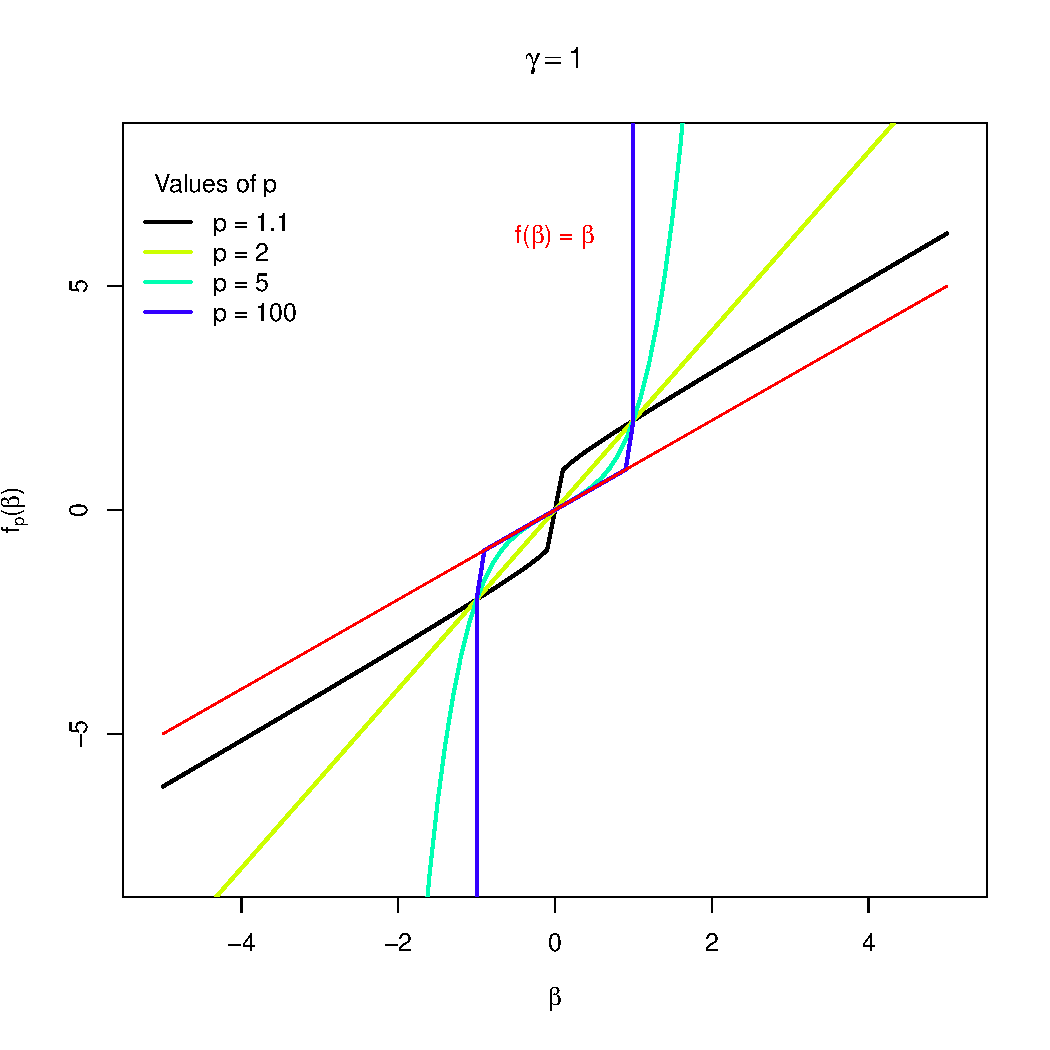
\includegraphics[width=\linewidth]{Images/Figures_Exercise_1/penal_1.pdf} % Replace with your first image file name
    \caption{$f_{p, \gamma}(\beta_i)$ for $\gamma = 1$}
    \label{fig:penal_1}
  \end{subfigure}
  \hfill
  \begin{subfigure}{0.45\textwidth}
    \centering
    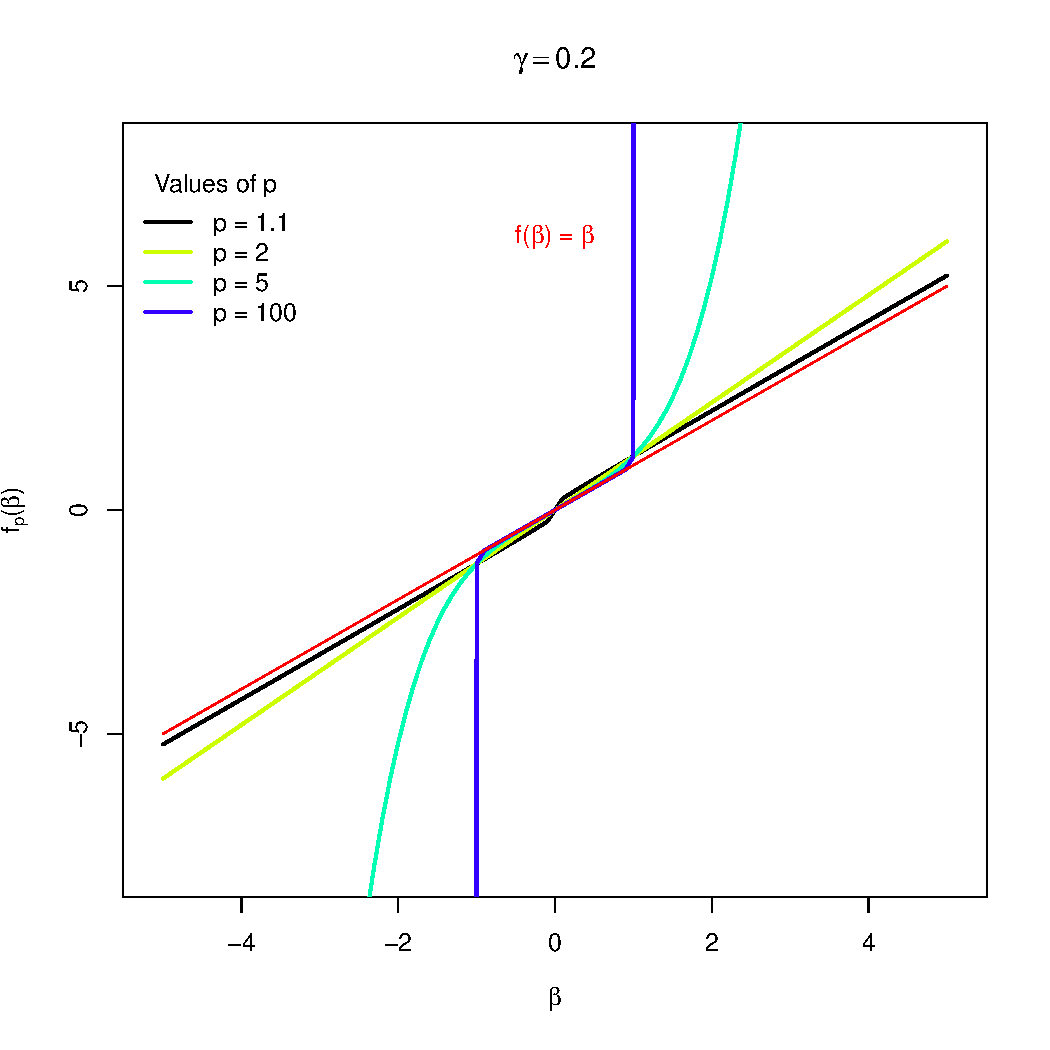
\includegraphics[width=\linewidth]{Images/Figures_Exercise_1/penal_2.pdf} % Replace with your second image file name
    \caption{$f_{p, \gamma}(\beta_i)$ for $\gamma = 0.2$}
    \label{fig:penal_2}
  \end{subfigure}
  \caption{Plots of $f_{p, \gamma}(\beta_i)$ where $f(\beta) = \beta$ is added for reference}
  \label{fig:penalized_lsq}
\end{figure}
with the respective inverse functions
\begin{figure}[H]
  \centering
  \begin{subfigure}{0.45\textwidth}
    \centering
    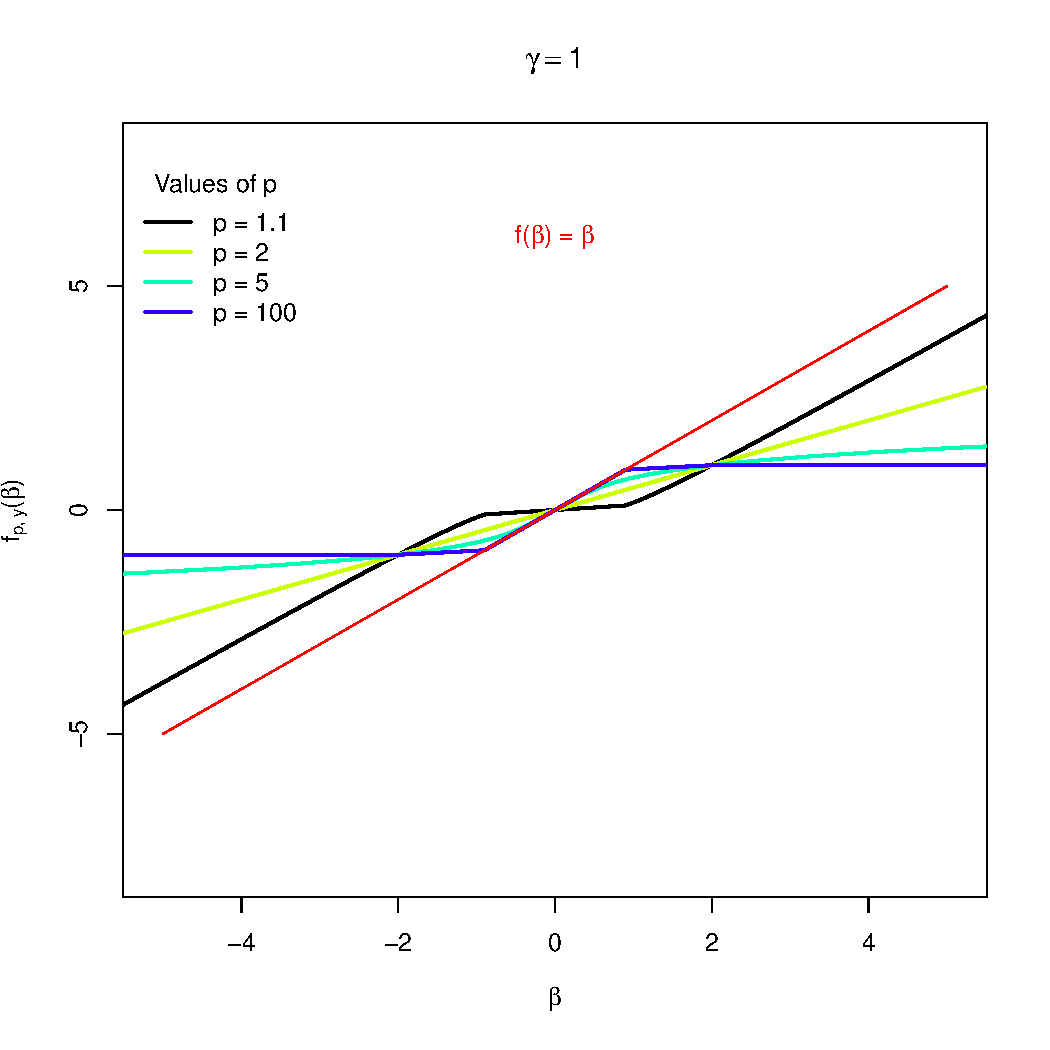
\includegraphics[width=\linewidth]{Images/Figures_Exercise_1/inverse_function_1.pdf} % Replace with your first image file name
    \caption{$f_{p, \gamma}^{-1}(\beta_i)$ for $\gamma = 1$}
    \label{fig:inv_1}
  \end{subfigure}
  \hfill
  \begin{subfigure}{0.45\textwidth}
    \centering
    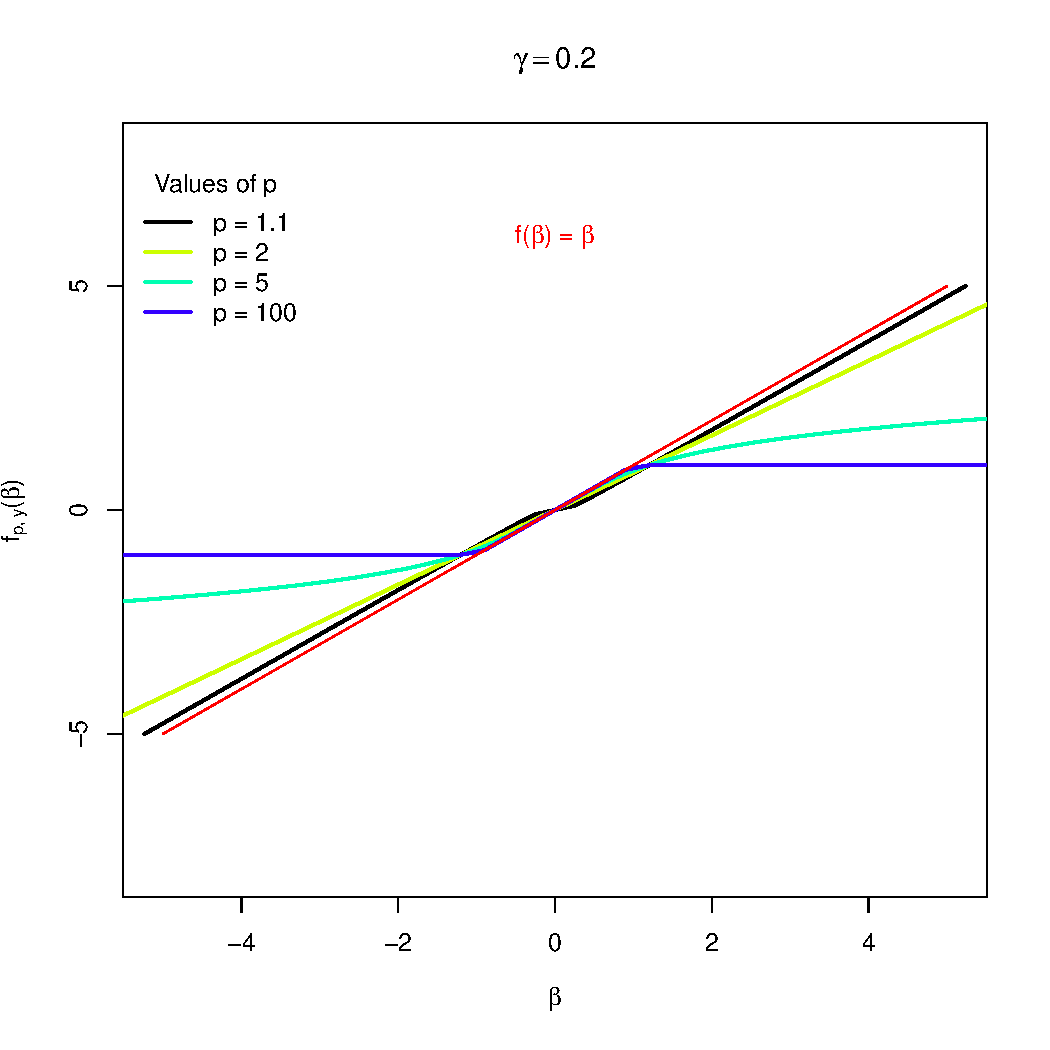
\includegraphics[width=\linewidth]{Images/Figures_Exercise_1/inverse_function_0.2.pdf} % Replace with your second image file name
    \caption{$f_{p, \gamma}^{-1}(\beta_i)$ for $\gamma = 0.2$}
    \label{fig:inv_0.2}
  \end{subfigure}
  \caption{Plots of the inverse of $f_{p. \gamma}(\beta_i)$ where $f(\beta) = \beta$ is added for reference}
  \label{fig:penalized_lsq_inv}
\end{figure}
The constant $\gamma$ determines the impact of the penalty term on the function $f$. When $\gamma$ equals zero, the penalty term is eliminated, resulting in a straight line. As $\gamma$ increases, the regularization effect becomes more pronounced.

The $p$-value influences the type of $L_p$-norm used for regularization. Higher $p$-values lead to a greater penalty for $\beta$ values larger than 1 in absolute value, while smaller $p$-values result in a lesser penalty, as raising $\beta$ to the $p$th power tends toward zero for large $p$-values.

Overall, higher $p$-values result in a heavier penalty for large $\beta$ values, and the $\gamma$ parameter allows control over the overall magnitude of this penalty term.
\nssection{d.)}
\emph{Implement a function which finds the root of expression (3). Use the method of bisection (book page 23). The root of (3) will be the estimator $\hat{\beta}_{\gamma, p}(y)$. What are good starting values for upper and lower bounds (in general)? Test the algorithm for $\gamma = 1$, and $p = 1.1$, $p = 2$, and $p = 100$. Evaluate the results for $y$ in the interval $[-5, 5]$, and plot the results in the same form as in c.)} \spaze 
\textbf{Solution:} \spaze
The implementation can be found in Appendix \ref{appendix:b}, from code listing  (\ref{lst:bisection}). It produces the following plot: 
\begin{figure}[H]
  \centering
  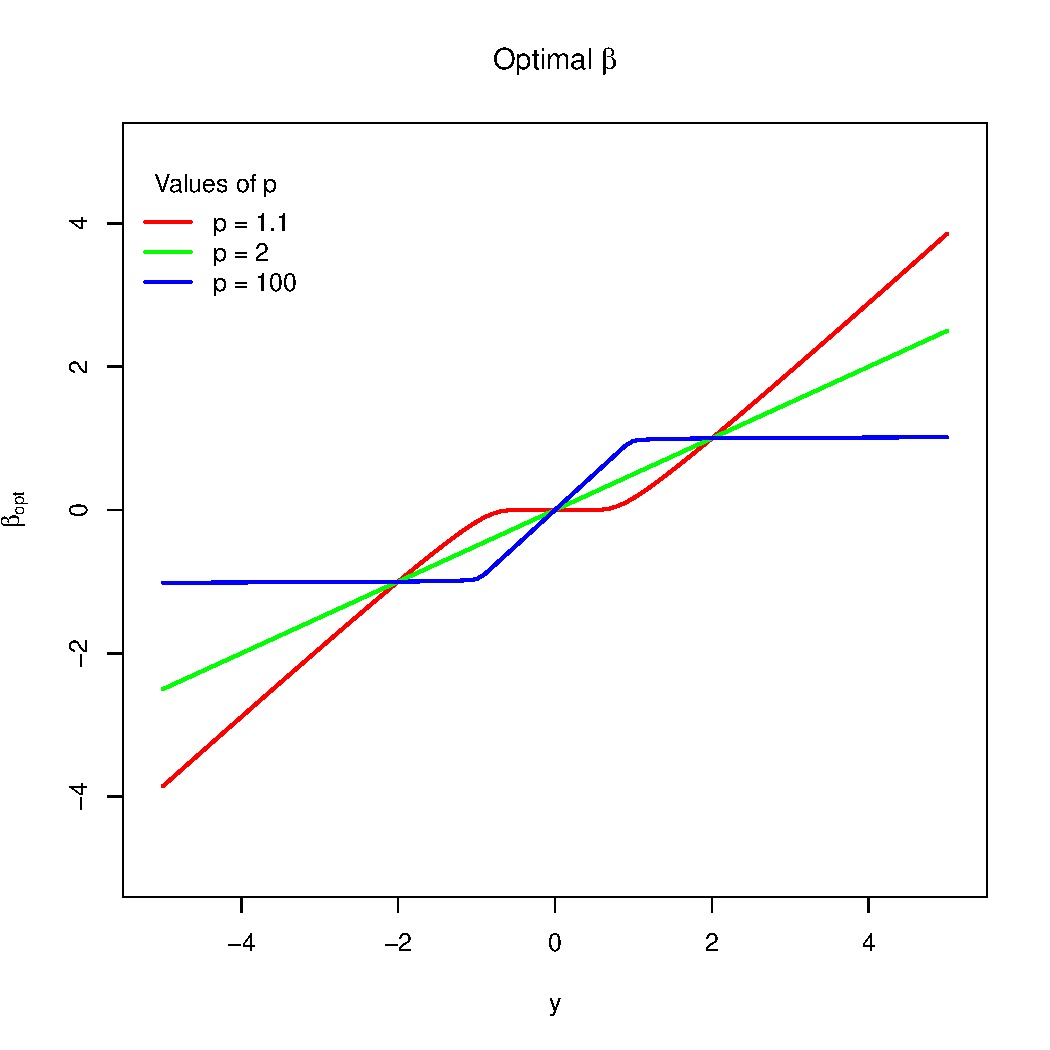
\includegraphics[width=0.6\textwidth]{Images/Figures_Exercise_1/bisection_plots.pdf}
  \caption{Finding the solution to $f_{p, \gamma}(\beta_i) = 0$ through the bisection method}
  \label{fig:example}
\end{figure}
Sensible starting values for upper and lower bounds for the bisection method would be $\mathcal{O}_{\beta} = |\beta|$ and $\Omega_{\beta} = -|\beta| $ respectively. Meaning then for some $\beta_0 \in (\Omega_{\beta} , \mathcal{O}_{\beta})$ we could be more assured to reach a solution.
\nssection{e.)}
\emph{Use the data set} \texttt{sparseDataWithErrors.dat} \emph{and perform estimation of parameters $\beta_i, i=1, \ldots, n$, from the data $y_i, i=1, \ldots, n$. Compare the result to the ground truth in terms of residual sum of squares. Do the estimation for penalized regression, i.e. compute $\hat{\beta}_{\gamma, p}$ with $\gamma=1, p=1.1, p=2$ and $p=100$, compare also to the MLE estimator. For $p=$ 100, try also to estimate the parameters $\beta_i$ by using the residuals, i.e. $\hat{\beta}_{1,100}^{\text {Alt }}=y-\hat{\beta}_{1,100}$. Comment on the results. How does MLE measure up?} \spaze 
\textbf{Solution:} \spaze 
The implementation can be found in Appendix \ref{appendix:b}, from code listing  (\ref{lst:bisection_est}). The estimation gives:
\begin{table}[H]
\centering
\begin{tabular}{SS} \toprule
{$p$} & {$\hat{\beta}_{1, 100}$} \\ \midrule
1.1 & 273.9674 \\ \hline
2.0 & 1256.5316 \\ \hline 
100.0 & 3786.6181 \\ \hline
\end{tabular}
\caption{Residuals for penalized regression}
\end{table}

\begin{table}[H]
\centering
\begin{tabular}{SS} \toprule
{$p$} & {$\hat{\beta}_{1, 100}^{\text{Alt}}$} \\ \midrule
1.1 & 3590.8957 \\ \hline
2.0 & 1256.5316 \\ \hline
100.0 & 251.9418 \\ \hline
\end{tabular}
\caption{Residuals for Alternative Estimation}
\label{tab:residuals_alternative}
\end{table}
The residual sum of squares of the MLE, $\text{RSS} \left(\hat{\theta}_{\text{MLE}} \right)$, gives 998.4152. Comparing the results, we find that the most accurate estimate for $\hat{\beta}_{1, 100}^{\text{Alt}}$ occurs at $p = 100$, yielding the lowest residual error. Following closely, the second-best estimate for $\hat{\beta}_{1, 100}$ comes at $p = 1.1$.
\nssection{f.)}
\emph{In the linear regression problem for $p=n$, we have data on the form:}
$$
\boldsymbol{y}=\boldsymbol{X} \boldsymbol{\beta}+\varepsilon
$$ \emph{Where $\boldsymbol{y}$ is the $(n \times 1)$ data vector, $\boldsymbol{\beta}$ is the $(n \times 1)$ parameter vector, $\boldsymbol{X}$ is a $(n \times n)$ design matrix, and $\boldsymbol{\varepsilon}$ is the $(n \times 1)$ error vector, with $\boldsymbol{\varepsilon} \sim \mathcal{N}(\mathbf{0}, I)$. How can you use the ADMM algorithm together with the solution to the problem above to derive a solution to the penalized regression problem?}
$$
\min _\beta\left\{-\ell(\boldsymbol{\beta} | \boldsymbol{y}, \boldsymbol{X})+\frac{\gamma}{p}\|\boldsymbol{\beta}\|_p^p\right\}
$$
\textbf{Solution:} \spaze
To derive a solution through the ADMM algorithm for the objective function
\[
\min_{\beta}\left\{-\ell(\boldsymbol{\beta} | \boldsymbol{y}, \boldsymbol{X}) + \frac{\gamma}{p}\|\boldsymbol{\beta} \|_p^p\right\}
\]
where \(\boldsymbol{y} = \boldsymbol{X} \boldsymbol{\beta} + \varepsilon\) and \(\varepsilon\) is a standard normal distributed variable, one can proceed as follows
\begin{enumerate}
  \item \textbf{Objective Function}: Start by defining the objective function, where as we know \(- \ell(\boldsymbol{\beta} | \boldsymbol{y}, \boldsymbol{X})\) represents the negative log-likelihood term, but is additionally conditioned on the data $\boldsymbol{X}$:
    \[
    \min_{\beta}\left\{-\ell(\boldsymbol{\beta} | \boldsymbol{y}, \boldsymbol{X}) + \frac{\gamma}{p}\|\boldsymbol{\beta}\|_p^p\right\}
    \]
    
  \item \textbf{Introduction of Auxiliary Variable}: Introduce an auxiliary variable \(\boldsymbol{\lambda}\) such that the problem becomes separable:
  $$
    \min_{\beta}\left\{-\ell(\boldsymbol{\beta} | \boldsymbol{y}, \boldsymbol{X}) + \frac{\gamma}{p}\|\boldsymbol{\lambda}\|_p^p\right\} $$
    $$\text{subject to} \quad \boldsymbol{\beta} = \boldsymbol{\lambda} \iff \boldsymbol{\beta} - \boldsymbol{\lambda}  = 0$$
  \item \textbf{Augmented Lagrangian}: We form the augmented Lagrangian function, combining the objective function and the constraint using a scaled dual variable \(\boldsymbol{u}\) (or the Lagrange multiplier):
    \[
    L_{\rho}(\boldsymbol{\beta}, \boldsymbol{\lambda}, \boldsymbol{u}) = -\ell(\boldsymbol{\beta} | \boldsymbol{y}, \boldsymbol{X}) + \frac{\gamma}{p}\|\boldsymbol{\lambda}\|_p^p + \boldsymbol{u}^T(\boldsymbol{\beta} - \boldsymbol{\lambda}) + \frac{\rho}{2} \lVert \boldsymbol{\beta} - \boldsymbol{\lambda} \rVert_{2}^2
    \]
  
  \item \textbf{ADMM Iterations}: We alternate between updating \(\boldsymbol{\beta}\), \(\boldsymbol{\lambda}\), and \(\boldsymbol{u}\) until convergence:
    \begin{itemize}
    \item \textbf{Update \( \boldsymbol{\beta} \)}:
   
    \[
    \boldsymbol{\beta}^{(k+1)} = \arg \min_{\boldsymbol{\beta}} \left\{-\ell(\boldsymbol{\beta} \mid \boldsymbol{y}, \boldsymbol{X}) + \frac{\rho}{2}\|\boldsymbol{\beta} - \boldsymbol{\lambda}^{(k)} + \boldsymbol{u}^{(k)}\|^2\right\}
    \]

    \item \textbf{Update \( \boldsymbol{\lambda} \)}:

    \[
    \boldsymbol{\lambda}^{(k+1)} = \arg \min_{\boldsymbol{\lambda}} \left\{\frac{\boldsymbol{\gamma}}{p}\|\boldsymbol{\lambda}\|_p^p + \frac{\rho}{2}\|\boldsymbol{\beta}^{(k+1)} - \boldsymbol{\lambda} + \boldsymbol{u}^{(k)}\|^2\right\}
    \]

    \item \textbf{Update \( \boldsymbol{u} \)}:

    \[
    \boldsymbol{u}^{(k+1)} = \boldsymbol{u}^{(k)} + \rho (\boldsymbol{\beta}^{(k+1)} - \boldsymbol{\lambda}^{(k+1)})
    \]
    \end{itemize}
  \item \textbf{Convergence}: We check for convergence based on the magnitude of the primal and dual residuals.
\end{enumerate}